% FIG ch03-03 three candidates with reading-order circles (Chinese)
\begin{tikzpicture}[font=\sffamily\small, text=BookInk]
  \tikzset{
    ord/.style={
      circle, draw=orange!85!black, line width=0.6pt, fill=orange!15,
      inner sep=1pt, font=\bfseries\footnotesize,
    },
  }
  \node[inner sep=0, anchor=south west] (A) at (0,0.38\linewidth) {%
    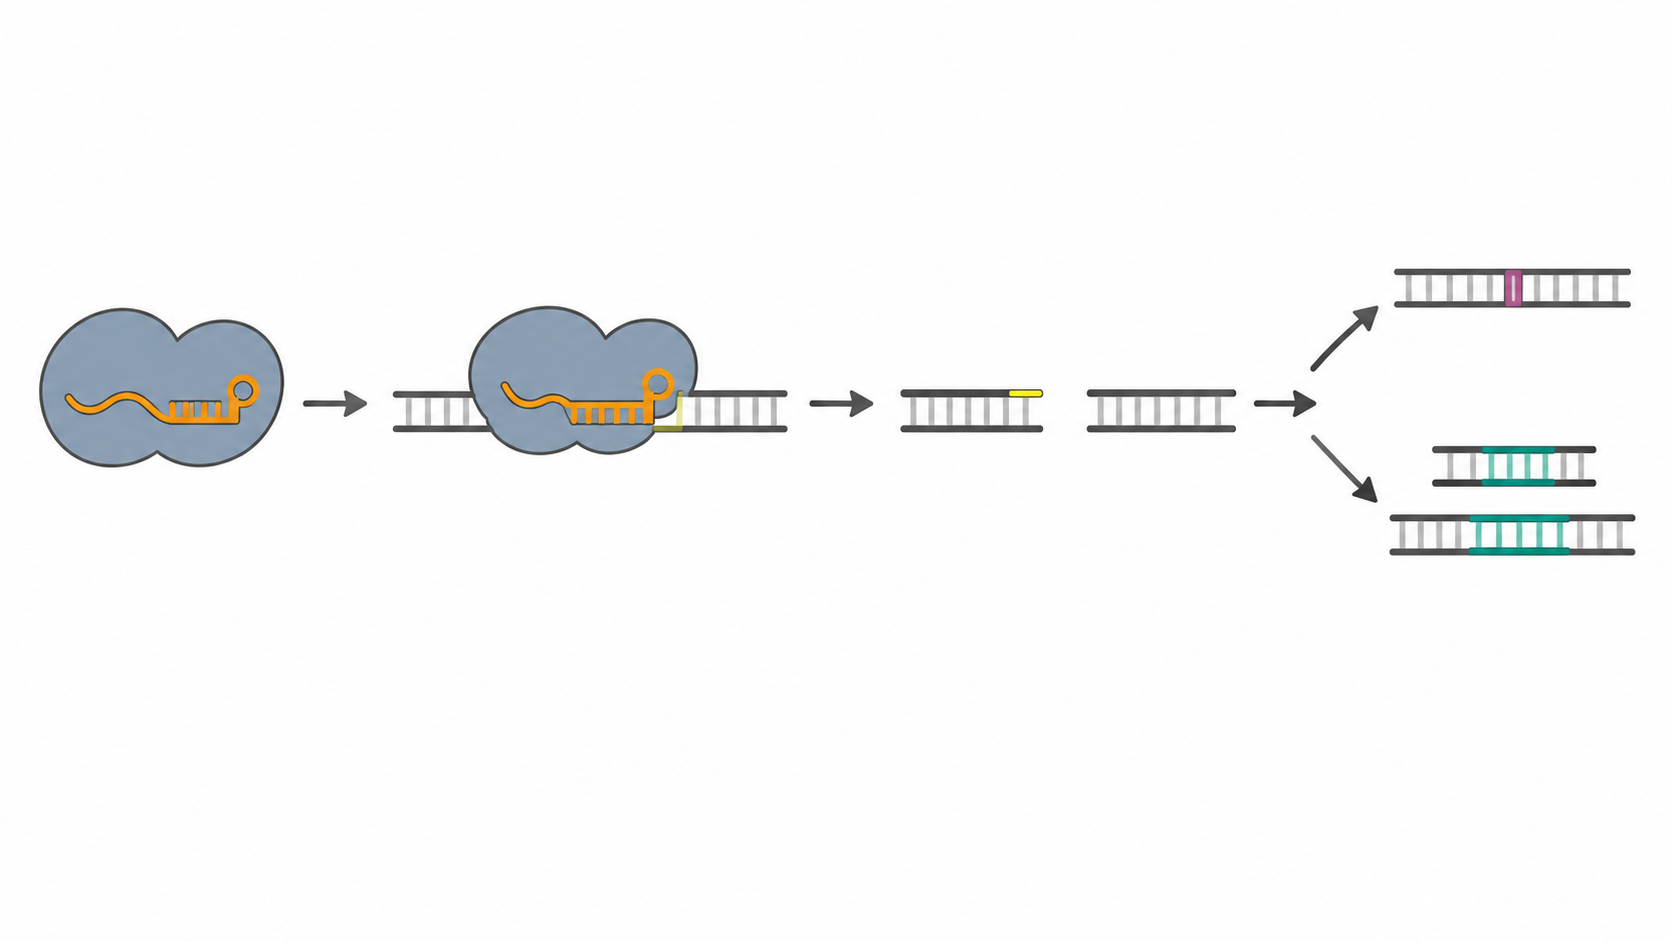
\includegraphics[width=0.32\linewidth]{figures/ch03/ch03-03a-cand-linear.png}};
  \node[inner sep=0, anchor=south west] (B) at (0.34\linewidth,0.38\linewidth) {%
    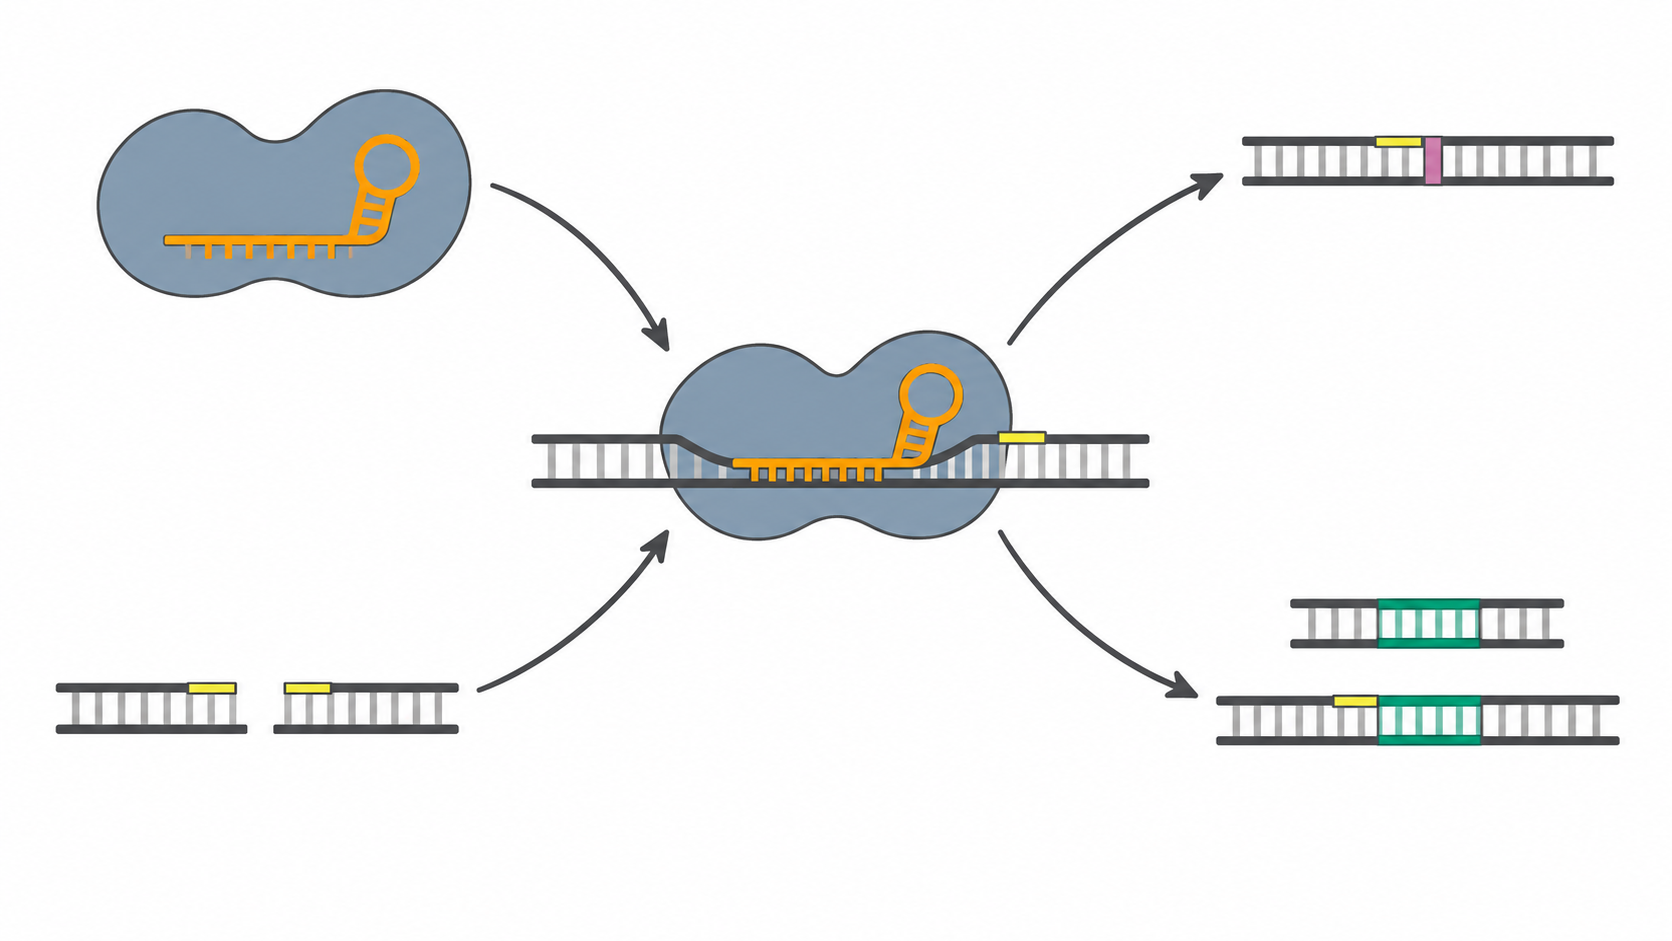
\includegraphics[width=0.32\linewidth]{figures/ch03/ch03-03b-cand-hub.png}};
  \node[inner sep=0, anchor=south west] (C) at (0.68\linewidth,0.38\linewidth) {%
    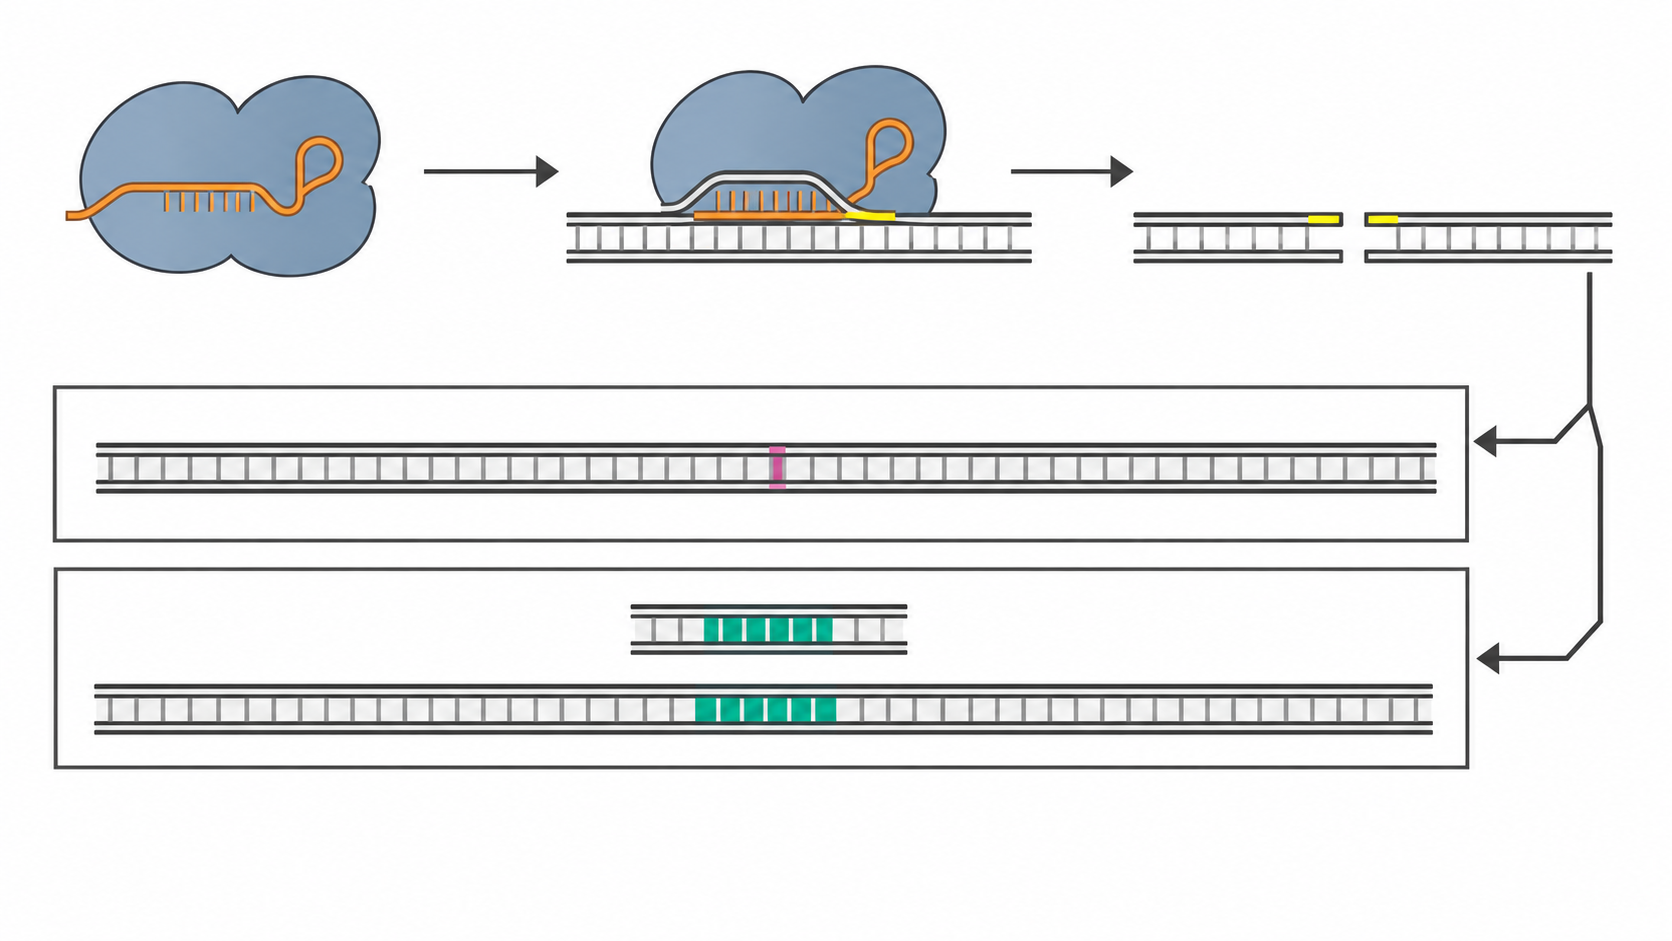
\includegraphics[width=0.32\linewidth]{figures/ch03/ch03-03c-cand-branch.png}};
  \node[font=\bfseries\Large, anchor=north west] at ($(A.north west)+(2mm,-2mm)$) {A};
  \node[font=\bfseries\Large, anchor=north west] at ($(B.north west)+(2mm,-2mm)$) {B};
  \node[font=\bfseries\Large, anchor=north west] at ($(C.north west)+(2mm,-2mm)$) {C};
  \begin{scope}[x={(A.south east)},y={(A.north west)}]
    \node[ord] at (0.08,0.55) {1};
    \node[ord] at (0.27,0.55) {2};
    \node[ord] at (0.46,0.55) {3};
    \node[ord] at (0.80,0.72) {4};
    \node[ord] at (0.80,0.35) {5};
  \end{scope}
  \begin{scope}[x={(C.south east)},y={(C.north west)}]
    \node[ord] at (0.15,0.85) {1};
    \node[ord] at (0.38,0.85) {2};
    \node[ord] at (0.62,0.85) {3};
    \node[ord] at (0.50,0.55) {4};
    \node[ord] at (0.50,0.22) {5};
  \end{scope}
\end{tikzpicture}
